\chapter{चीज़ें किससे बनी हैं}\label{ch:g1:materials-around-us}

नाश्ते की मेज़ को देखो। उस पर एक चम्मच है, दूध का एक गिलास है, एक
काँटा, एक नैपकिन, एक कटोरी है, और कुर्सी की पीठ पर एक स्वेटर टँगा है।
कितनी सारी चीज़ें! और हर चीज़ किसी न किसी चीज़ से बनी है: चम्मच लकड़ी
का, काँटा धातु का, गिलास काँच का, नैपकिन कागज़ का, कटोरी प्लास्टिक
की, स्वेटर ऊन का। मेज़ भर चीज़ें, पर बनी हैं गिनी-चुनी सामग्रियों से।
यह अध्याय इन्हीं सामग्रियों के बारे में है।

\begin{omfigure}
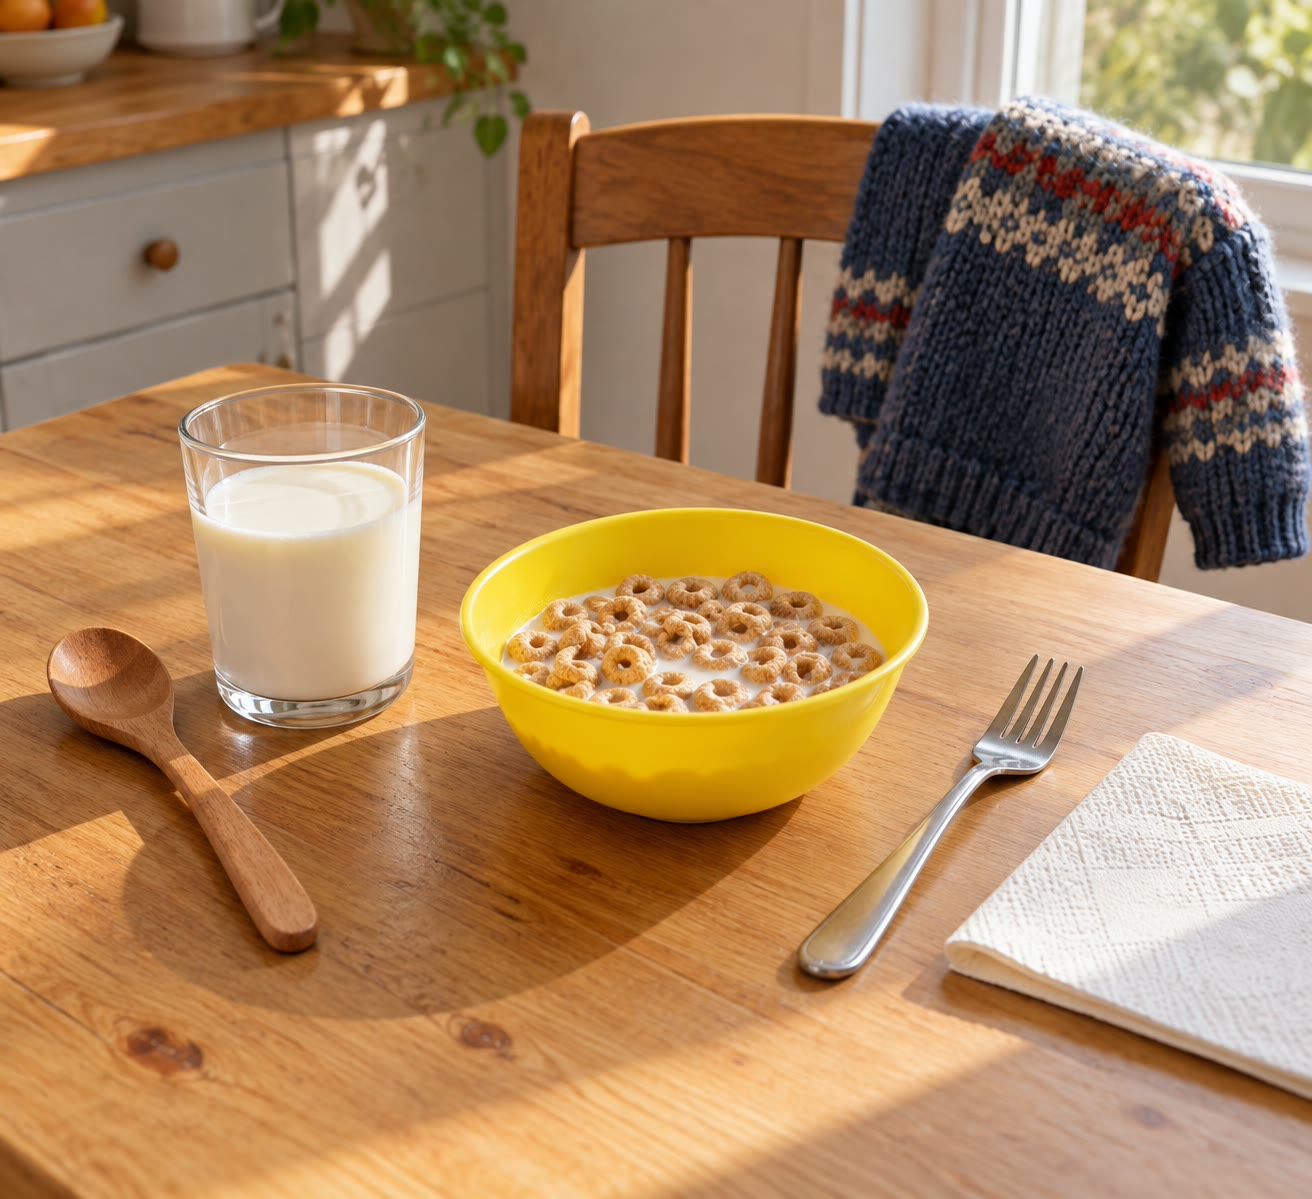
\includegraphics[width=0.62\linewidth]{images/book1/ai/g1-breakfast-table.jpg}

{\small नाश्ते की मेज़: बहुत-सी वस्तुएँ, थोड़ी-सी सामग्रियों से बनी।}
\end{omfigure}

\section{वस्तुएँ और सामग्रियाँ}

\begin{definition}[वस्तु]\label{def:g1:materials-around-us:object}
\emph{वस्तु}\index{वस्तु} वह चीज़ है जिसे हम देख और छू सकते हैं, और
अक्सर हाथ में पकड़कर काम में ले सकते हैं: चम्मच, कुर्सी, गेंद, खिड़की, जूता।
\end{definition}

\begin{definition}[सामग्री]\label{def:g1:materials-around-us:material}
किसी \omterm{def:g1:materials-around-us:object}{वस्तु} की \emph{सामग्री}\index{सामग्री} वह है जिससे वह \omterm{def:g1:materials-around-us:object}{वस्तु}
बनी है। चम्मच लकड़ी का, धातु का या प्लास्टिक का बन सकता है: चम्मच
\omterm{def:g1:materials-around-us:object}{वस्तु} है, लकड़ी उसकी सामग्री है।
\end{definition}

\begin{example}[एक वस्तु, तीन सामग्रियाँ]\label{ex:g1:materials-around-us:spoons}
तीन चम्मच अगल-बगल रखे हैं। उनका आकार एक जैसा है और वे एक ही काम
करते हैं, इसलिए वे एक ही तरह की \omterm{def:g1:materials-around-us:object}{वस्तु} हैं। पर एक लकड़ी का है, एक
धातु का और एक प्लास्टिक का: तीन अलग-अलग सामग्रियाँ।
\end{example}

\begin{omfigure}
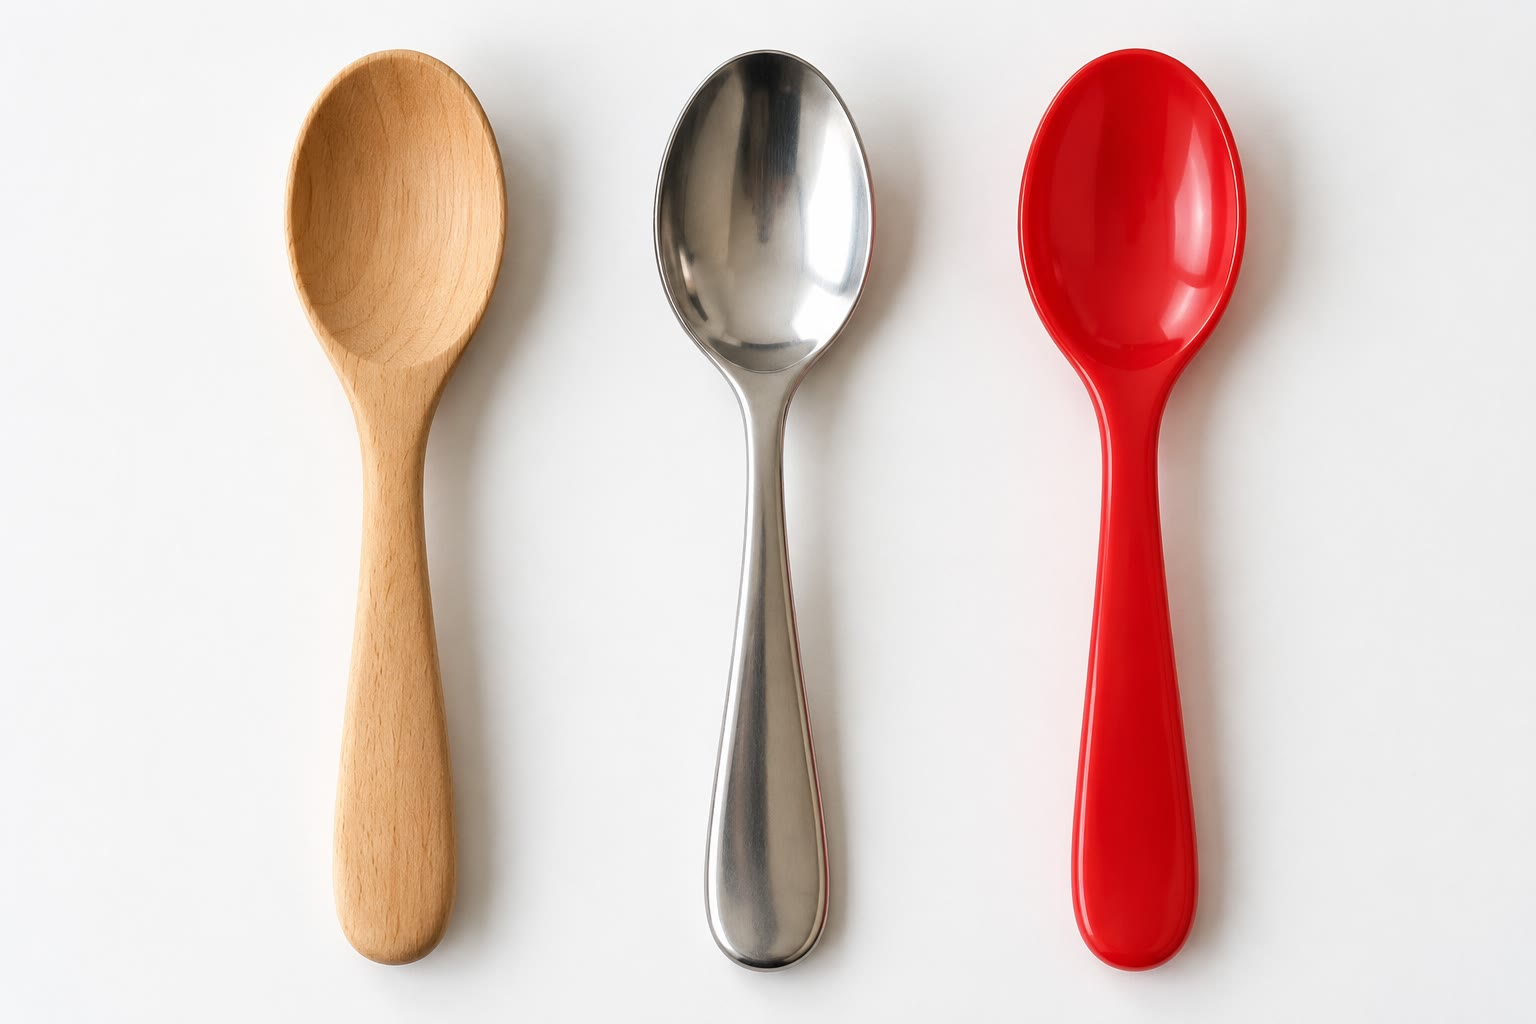
\includegraphics[width=0.55\linewidth]{images/book1/ai/g1-three-spoons.jpg}

{\small तीन चम्मच: एक ही \omterm{def:g1:materials-around-us:object}{वस्तु}, तीन सामग्रियाँ --- लकड़ी, धातु
और प्लास्टिक।}
\end{omfigure}

\begin{example}[एक सामग्री, अनेक वस्तुएँ]\label{ex:g1:materials-around-us:wood}
पेंसिल, कुर्सी, दरवाज़ा, खिलौना रेलगाड़ी और लकड़ी का चम्मच --- इन सबकी
\omterm{def:g1:materials-around-us:material}{सामग्री} लकड़ी है। एक ही \omterm{def:g1:materials-around-us:material}{सामग्री} से बहुत-सी अलग-अलग वस्तुएँ बन सकती हैं।
\end{example}

\begin{remark}[कई सामग्रियों से बनी वस्तुएँ]\label{rem:g1:materials-around-us:several}
बहुत-सी वस्तुएँ एक से ज़्यादा सामग्रियों से बनी होती हैं। कैंची के
फल धातु के होते हैं और हत्थे प्लास्टिक के। पेंसिल बाहर से लकड़ी की
होती है और अंदर ग्रेफ़ाइट की एक धूसर छड़ होती है। खिड़की में काँच
होता है, और उसका चौखटा लकड़ी, धातु या प्लास्टिक का होता है।
\end{remark}

\section{सात आम सामग्रियाँ}

\begin{proposition}[हमारे चारों ओर की सामग्रियाँ]\label{prop:g1:materials-around-us:seven}
हमारे आस-पास की ज़्यादातर वस्तुएँ कुछ आम सामग्रियों से बनी हैं:
\begin{itemize}
  \item \textbf{लकड़ी}: मेज़, कुर्सियाँ, पेंसिलें, दरवाज़े;
  \item \textbf{धातु}: काँटे, चाबियाँ, कीलें, कड़ाहियाँ, साइकिलें;
  \item \textbf{काँच}: खिड़कियाँ, मर्तबान, बोतलें, गिलास;
  \item \textbf{प्लास्टिक}: कटोरियाँ, बोतलें, खिलौने, बाल्टियाँ;
  \item \textbf{कागज़} और गत्ता: किताबें, नैपकिन, डिब्बे;
  \item \textbf{कपड़ा}: पहनने के कपड़े, परदे, थैले --- ऊन, सूत
        या दूसरे धागों से बने;
  \item \textbf{पत्थर}: दीवारें, सीढ़ियाँ, कंकड़, मूर्तियाँ।
\end{itemize}
\end{proposition}

\begin{omfigure}
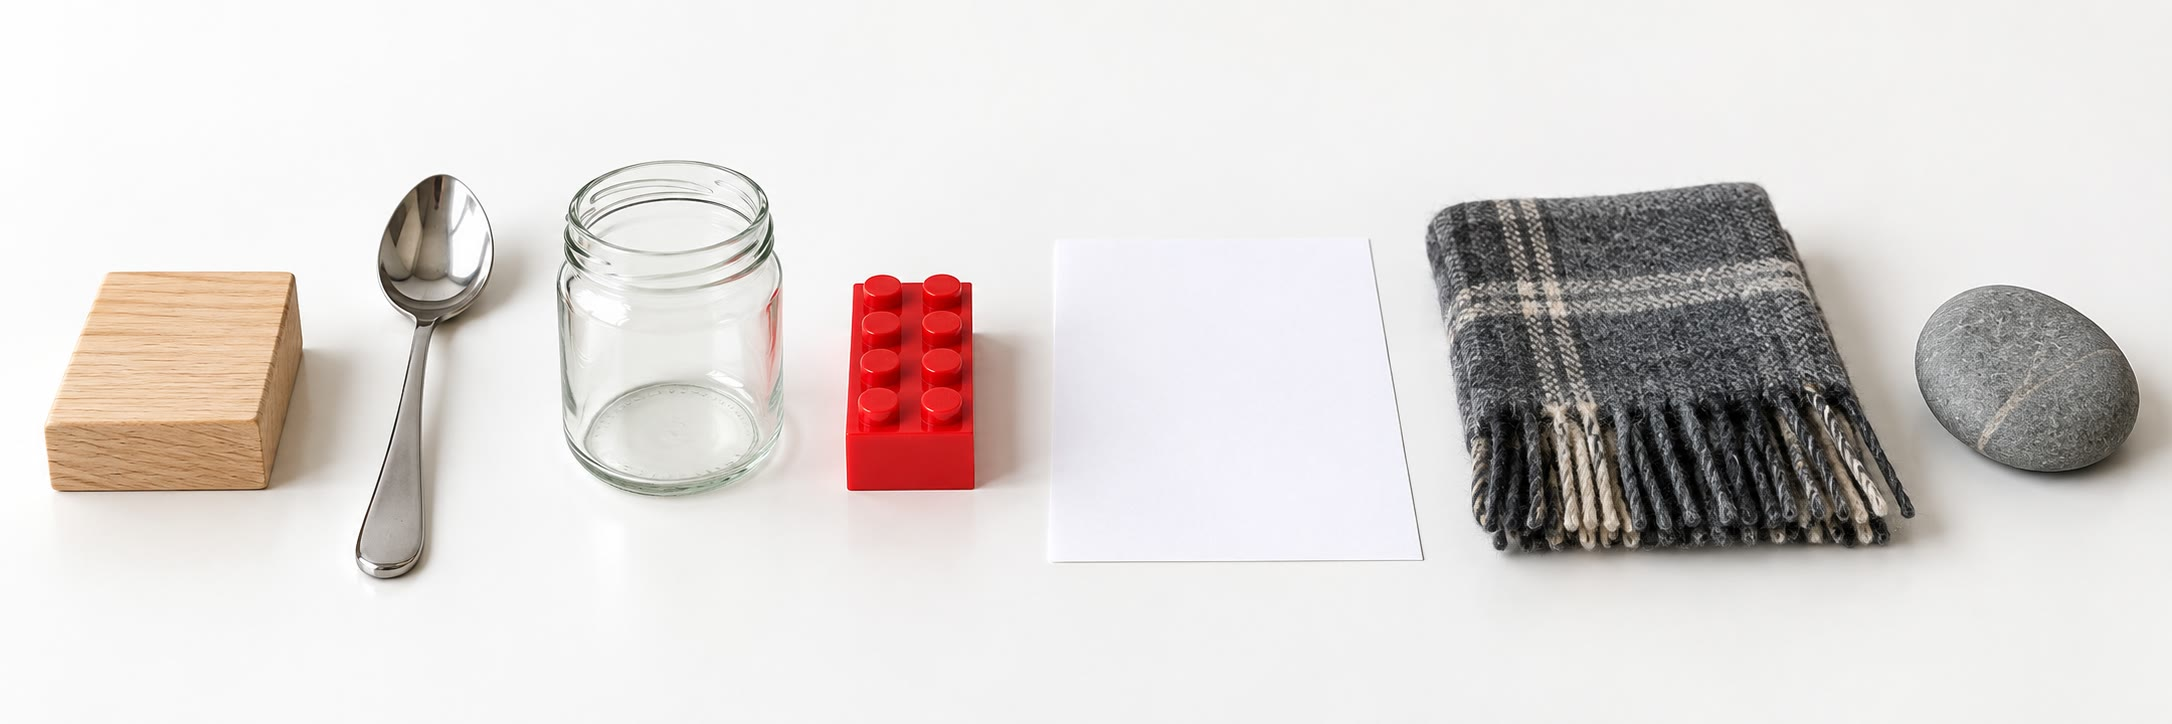
\includegraphics[width=0.75\linewidth]{images/book1/ai/g1-material-samples.jpg}

{\small सात नमूने, बाएँ से दाएँ: लकड़ी, धातु, काँच, प्लास्टिक,
कागज़, कपड़ा (ऊन) और पत्थर।}
\end{omfigure}

\begin{remark}[ऐसे नाम जो सामग्रियों के भी हैं]\label{rem:g1:materials-around-us:names}
पानी पीने के गिलास को हम ``काँच का गिलास'' कहते हैं, और कभी-कभी बस
``काँच'' भी, क्योंकि वह काँच से बना है। तब \omterm{def:g1:materials-around-us:object}{वस्तु} का नाम और \omterm{def:g1:materials-around-us:material}{सामग्री}
का नाम एक ही हो जाता है। जब हम सामग्रियों की बात करते हैं, तो हमारा
मतलब उस चीज़ से होता है जिससे \omterm{def:g1:materials-around-us:object}{वस्तु} बनी है, \omterm{def:g1:materials-around-us:object}{वस्तु} से नहीं।
\end{remark}

\section{सामग्रियों के गुण}

\begin{definition}[सामग्री का गुण]\label{def:g1:materials-around-us:property}
\emph{सामग्री का गुण}\index{सामग्री का गुण} वह बात है जो हम उसे देखकर,
छूकर या परखकर जान सकते हैं: क्या वह कठोर है या नरम? क्या हम उसके
आर-पार देख सकते हैं? क्या चुंबक उसे खींचता है? क्या वह पानी पर
तैरती है या डूब जाती है?
\end{definition}

\begin{example}[कठोर और नरम]\label{ex:g1:materials-around-us:hard}
कंकड़ कठोर होता है: अँगूठे से दबाने पर उस पर कोई निशान नहीं पड़ता।
ऊन का मफ़लर नरम होता है: वह हाथ में मुड़ता और तह होता है। लकड़ी, धातु,
काँच और पत्थर कठोर हैं; कपड़ा और कागज़ नरम हैं और आसानी से मुड़ते हैं।
\end{example}

\begin{example}[आर-पार देखना]\label{ex:g1:materials-around-us:see-through}
खिड़की से हम बगीचा देख सकते हैं: काँच प्रकाश को आर-पार जाने देता है,
हम कहते हैं कि वह \emph{पारदर्शी} है। लकड़ी के दरवाज़े, ईंट की दीवार
या धातु की कड़ाही के आर-पार हम नहीं देख सकते। कुछ प्लास्टिक पारदर्शी
होते हैं, जैसे पानी की बोतल; कुछ नहीं होते, जैसे खिलौने की लाल ईंट।
\end{example}

\begin{example}[चुंबक से खिंचना]\label{ex:g1:materials-around-us:magnet}
चुंबक स्टील की पेपर-क्लिप, स्टील की कील या लोहे की चाबी को अपनी ओर
खींच लेता है। वह लकड़ी, काँच, प्लास्टिक, कागज़, कपड़े या पत्थर को
नहीं खींचता। और, हैरानी की बात है कि वह हर धातु को भी नहीं खींचता:
ऐलुमिनियम का पेय-डिब्बा और ताँबे का तार अपनी जगह पड़े रहते हैं। चुंबक
लोहे की और स्टील की वस्तुओं को खींचता है; स्टील ज़्यादातर लोहा ही है।
\end{example}

\begin{omfigure}
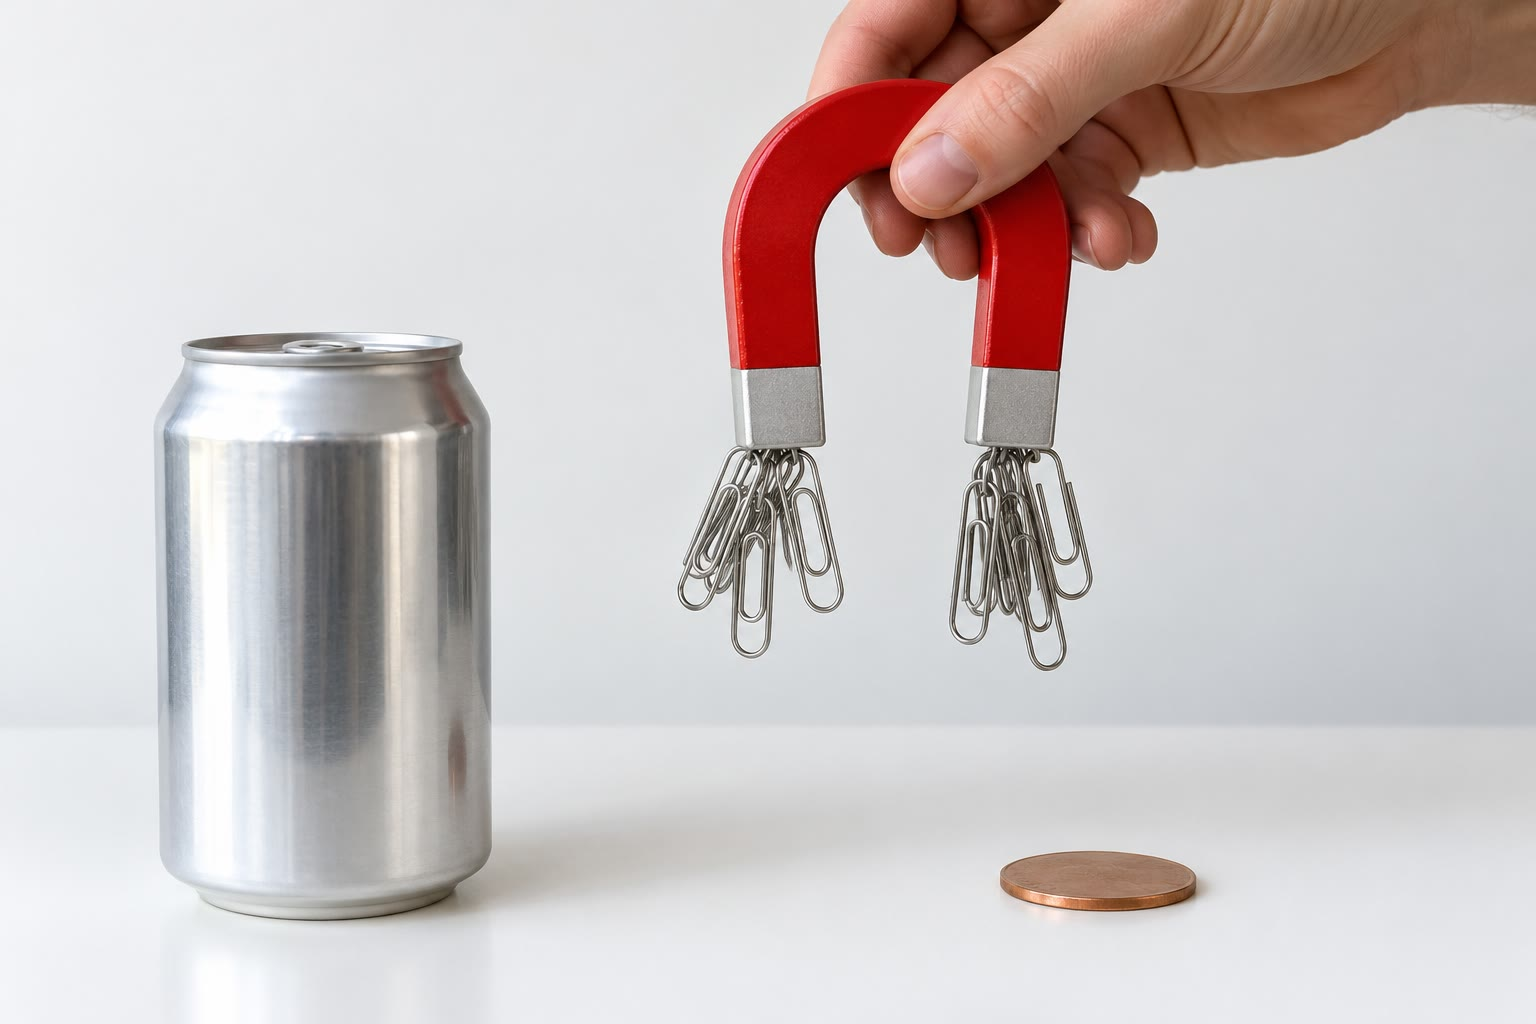
\includegraphics[width=0.55\linewidth]{images/book1/ai/g1-magnet-clips.jpg}

{\small चुंबक स्टील की पेपर-क्लिपें उठा लेता है। मेज़ पर रखा ऐलुमिनियम
का डिब्बा और ताँबे की चकती अपनी जगह पड़े रहते हैं।}
\end{omfigure}

\begin{example}[तैरना और डूबना]\label{ex:g1:materials-around-us:float}
पानी के एक टब में कुछ वस्तुएँ डालो। लकड़ी का गुटका और प्लास्टिक की
बोतल का ढक्कन तैरते हैं। कंकड़, काँच का कंचा और स्टील की कील तली में
डूब जाते हैं। कोई चीज़ तैरती है या डूबती है, यह भी उसकी \omterm{def:g1:materials-around-us:material}{सामग्री} का
एक गुण है।
\end{example}

\begin{omfigure}
\begin{tikzpicture}[font=\small]
  % the basin
  \fill[omWater!80] (0,0) rectangle (9,2.2);
  \draw[omGlass, line width=0.8pt] (-0.1,2.7) -- (0,2.6) -- (0,0) -- (9,0)
    -- (9,2.6) -- (9.1,2.7);
  % floating: wooden block, plastic cap
  \fill[brown!55, draw=brown!70!black] (0.8,2.0) rectangle (2.2,2.5);
  \fill[red!70, draw=red!50!black] (3.7,2.05) rectangle (4.3,2.35);
  % sunk: pebble, marble, nail
  \fill[black!35, draw=black!60] (5.0,0.25) ellipse (0.45 and 0.22);
  \shade[ball color=cyan!40] (6.5,0.2) circle (0.18);
  \fill[black!55] (7.6,0.06) rectangle (8.6,0.14);
  \fill[black!55] (7.52,0.02) rectangle (7.62,0.18);
  % labels
  \node[anchor=south] at (1.5,2.75) {लकड़ी का गुटका};
  \node[anchor=south] at (4.0,2.75) {प्लास्टिक ढक्कन};
  \node[anchor=north] at (5.0,-0.1) {कंकड़};
  \node[anchor=north] at (6.5,-0.1) {कंचा};
  \node[anchor=north] at (8.1,-0.1) {कील};
  \node[anchor=west, align=left] at (9.3,2.2) {ये तैरते हैं};
  \node[anchor=west, align=left] at (9.3,0.2) {ये डूबते हैं};
\end{tikzpicture}

{\small पानी के टब में: लकड़ी का गुटका और प्लास्टिक का ढक्कन तैरते हैं;
कंकड़, काँच का कंचा और स्टील की कील डूब जाते हैं।}
\end{omfigure}

\section{सामग्रियों को छाँटना}

\begin{method}[एक गुण से छाँटना]\label{met:g1:materials-around-us:sort}
वस्तुओं के एक ढेर को छाँटने के लिए:
\begin{enumerate}
  \item \textbf{एक} सवाल चुनो, जैसे ``क्या चुंबक इसे खींचता
        है?'';
  \item हर \omterm{def:g1:materials-around-us:object}{वस्तु} को परखो और उसे ``हाँ'' वाले ढेर में या ``नहीं'' वाले
        ढेर में रखो;
  \item फिर, चाहो तो, हर ढेर को किसी दूसरे सवाल से दोबारा छाँटो।
\end{enumerate}
एक बार में एक ही सवाल: इस तरह हर \omterm{def:g1:materials-around-us:object}{वस्तु} की ठीक एक ही जगह होती है।
\end{method}

\begin{omfigure}
\begin{tikzpicture}[font=\small]
  \draw[omDef, line width=1pt] (0,0) circle (2.3);
  \draw[omProp, line width=1pt] (2.4,0) circle (2.3);
  \node[omDef, font=\small\bfseries] at (-0.6,2.65) {धातु से बनी};
  \node[omProp, font=\small\bfseries] at (3.0,2.65) {चुंबक से खिंचती};
  \node[font=\footnotesize] at (-1.1,0.35) {पेय-डिब्बा};
  \node[font=\footnotesize] at (-1.1,-0.35) {ताँबे का तार};
  \node[font=\footnotesize] at (1.2,0.6) {स्टील की कील};
  \node[font=\footnotesize] at (1.2,0) {लोहे की चाबी};
  \node[font=\footnotesize] at (1.2,-0.6) {पेपर-क्लिप};
  \node[font=\footnotesize] at (3.5,0) {(कुछ नहीं)};
  \node[anchor=west] at (5.2,0.9) {लकड़ी का चम्मच};
  \node[anchor=west] at (5.2,0.3) {काँच का कंचा};
  \node[anchor=west] at (5.2,-0.3) {ऊन का मफ़लर};
  \node[anchor=west] at (5.2,-0.9) {कंकड़};
\end{tikzpicture}

{\small दो सवाल, दो घेरे। नीले घेरे के अंदर: धातु से बनी वस्तुएँ।
नारंगी घेरे के अंदर: वे वस्तुएँ जिन्हें चुंबक खींचता है। दोनों घेरों
में: लोहे या स्टील की वस्तुएँ। दोनों के बाहर: बाकी सब कुछ।}
\end{omfigure}

\begin{center}
\small
\begin{tabular}{lccc}
\hline
\omterm{def:g1:materials-around-us:object}{वस्तु} (\omterm{def:g1:materials-around-us:material}{सामग्री}) & कठोर? & आर-पार दिखता? & चुंबक से खिंचती? \\
\hline
गुटका (लकड़ी) & हाँ & नहीं & नहीं \\
कील (स्टील) & हाँ & नहीं & हाँ \\
कंचा (काँच) & हाँ & हाँ & नहीं \\
बोतल का ढक्कन (प्लास्टिक) & हाँ & नहीं & नहीं \\
पन्ना (कागज़) & नहीं & नहीं & नहीं \\
मफ़लर (ऊन) & नहीं & नहीं & नहीं \\
कंकड़ (पत्थर) & हाँ & नहीं & नहीं \\
\hline
\end{tabular}
\end{center}

\section{काम के लिए सही सामग्री}

\begin{proposition}[हर सामग्री अपने गुणों के कारण चुनी जाती है]\label{prop:g1:materials-around-us:choose}
लोग किसी \omterm{def:g1:materials-around-us:object}{वस्तु} की \omterm{def:g1:materials-around-us:material}{सामग्री} इस हिसाब से चुनते हैं कि उस \omterm{def:g1:materials-around-us:object}{वस्तु} को क्या काम करना है:
\begin{itemize}
  \item खिड़की को प्रकाश अंदर आने देना है: वह काँच की बनती है, जो
        पारदर्शी है;
  \item बरसाती को बारिश रोकनी है और तह भी होना है: वह प्लास्टिक की
        बनती है, या ऐसे कपड़े की जिसमें से पानी नहीं निकल सकता;
  \item कड़ाही चूल्हे पर पिघलनी नहीं चाहिए: वह धातु की बनती है;
  \item कड़ाही का हत्था हाथ नहीं जलाना चाहिए: वह अक्सर लकड़ी का या
        कठोर प्लास्टिक का बनता है, जो धातु जितने गरम नहीं होते;
  \item तकिया नरम होना चाहिए: वह कपड़े का बनता है, जिसमें पंख
        या रेशे भरे होते हैं।
\end{itemize}
\end{proposition}

\begin{example}[नाव]\label{ex:g1:materials-around-us:boat}
खिलौना नाव को तैरना है। वह लकड़ी की या प्लास्टिक की बन सकती है।
पत्थर के ठोस टुकड़े से बनी नाव तुरंत डूब जाएगी।
\end{example}

\begin{remark}[टूटा काँच]\label{rem:g1:materials-around-us:glass}
काँच कठोर है, पर टूट जाता है, और उसके टुकड़े नुकीले होते हैं। जब
काँच का गिलास टूटता है, तो टुकड़े कोई बड़ा व्यक्ति ही उठाता है।
\end{remark}

\section{अभ्यास}

\begin{exercise}[$\star$]\label{exo:g1:materials-around-us:1}
क्या कुर्सी \omterm{def:g1:materials-around-us:object}{वस्तु} है या \omterm{def:g1:materials-around-us:material}{सामग्री}? क्या लकड़ी \omterm{def:g1:materials-around-us:object}{वस्तु} है या \omterm{def:g1:materials-around-us:material}{सामग्री}?
\end{exercise}

\begin{exercise}[$\star$]\label{exo:g1:materials-around-us:2}
हर \omterm{def:g1:materials-around-us:object}{वस्तु} की \omterm{def:g1:materials-around-us:material}{सामग्री} बताओ: खिड़की का शीशा, कील, कंकड़,
किताब, मोज़ा।
\end{exercise}

\begin{exercise}[$\star$]\label{exo:g1:materials-around-us:3}
लकड़ी से बनी दो वस्तुएँ और प्लास्टिक से बनी दो वस्तुएँ बताओ।
\end{exercise}

\begin{exercise}[$\star$]\label{exo:g1:materials-around-us:4}
जो अलग है उसे ढूँढो, और बताओ क्यों: लकड़ी का चम्मच, धातु का काँटा,
प्लास्टिक का चम्मच, लकड़ी की कुर्सी। (सामग्रियों को देखो।)
\end{exercise}

\begin{exercise}[$\star$]\label{exo:g1:materials-around-us:5}
किस \omterm{def:g1:materials-around-us:material}{सामग्री} के आर-पार हम देख सकते हैं: लकड़ी, काँच या पत्थर?
\end{exercise}

\begin{exercise}[$\star$]\label{exo:g1:materials-around-us:6}
स्टील की एक कील, काँच का एक कंचा और लकड़ी का एक गुटका --- इनके पास
एक चुंबक लाया जाता है। वह किसे खींचता है?
\end{exercise}

\begin{exercise}[$\star$]\label{exo:g1:materials-around-us:7}
टब वाला चित्र देखो। कितनी वस्तुएँ तैरती हैं? कितनी
डूबती हैं?
\end{exercise}

\begin{exercise}[$\star$]\label{exo:g1:materials-around-us:8}
कैंची में फल होते हैं और हत्थे। हर हिस्सा किस \omterm{def:g1:materials-around-us:material}{सामग्री} का बना है?
कैंची एक \omterm{def:g1:materials-around-us:material}{सामग्री} से बनी है या दो से?
\end{exercise}

\begin{exercise}[$\star$]\label{exo:g1:materials-around-us:9}
दो घेरों वाला चित्र देखो। पेय-डिब्बा किस घेरे में है? वह नारंगी
घेरे में क्यों नहीं है?
\end{exercise}

\begin{exercise}[$\star\star$]\label{exo:g1:materials-around-us:10}
खिड़कियाँ काँच की क्यों बनती हैं, लकड़ी की क्यों नहीं?
\end{exercise}

\begin{exercise}[$\star\star$]\label{exo:g1:materials-around-us:11}
सैम इन 8 वस्तुओं को ``क्या चुंबक इसे खींचता है?'' वाले सवाल से छाँटना
चाहता है: स्टील की कील, पेपर-क्लिप, कंकड़, लकड़ी का चम्मच, लोहे की
चाबी, पेय-डिब्बा, काँच का कंचा, ऊन का मोज़ा। ``हाँ'' वाले ढेर में कितनी
वस्तुएँ जाएँगी? ``नहीं'' वाले ढेर में कितनी?
\end{exercise}
